% -*- latex -*-
%%%%%%%%%%%%%%%%%%%%%%%%%%%%%%%%%%%%%%%%%%%%%%%%%%%%%%%%%%%%%%%%
%%%%%%%%%%%%%%%%%%%%%%%%%%%%%%%%%%%%%%%%%%%%%%%%%%%%%%%%%%%%%%%%
%%%%
%%%% This text file is part of the source of 
%%%% `Parallel Computing'
%%%% by Victor Eijkhout, copyright 2012-9
%%%%
%%%% parcompbook.tex : master file for the book
%%%%
%%%%%%%%%%%%%%%%%%%%%%%%%%%%%%%%%%%%%%%%%%%%%%%%%%%%%%%%%%%%%%%%
%%%%%%%%%%%%%%%%%%%%%%%%%%%%%%%%%%%%%%%%%%%%%%%%%%%%%%%%%%%%%%%%

\documentclass[11pt,letterpaper,twoside,openany]{boek3}
%\documentclass{book}

\usepackage{verbatim}
\makeatletter
\def\verbatim@startline{\verbatim@line{\leavevmode\kern\unitindent\relax}}
\makeatother

\usepackage{comment}
\specialcomment{tacc}{\def\CommentCutFile{tacc.cut}}{}
\newif\ifIncludeAnswers
\IncludeAnswersfalse
\input inex
\includecomment{gpu}
\includecomment{review}
\includecomment{book}

\usepackage{graphicx,outliner,undertilde,wrapfig}

% fancy text stuff
\usepackage{dirtree,multicol,multirow,times}

% AMS math
\usepackage[fleqn]{amsmath}
\usepackage{amssymb}

% custom arrays and tables
\usepackage{array} %,multirow,multicol}
\newcolumntype{R}{>{\hbox to 1.2em\bgroup\hss}{r}<{\egroup}}
\newcolumntype{T}{>{\hbox to 8em\bgroup}{c}<{\hss\egroup}}

% algorithms
\usepackage[algo2e,noline,noend]{algorithm2e}
\newenvironment{displayalgorithm}
 {\begin{algorithm2e}[H]\leftskip=\unitindent \DontPrintSemicolon
  \SetKwInOut{Input}{Input}\SetKwInOut{Output}{Output}
 }
 {\end{algorithm2e}}
\newenvironment{displayprocedure}[2]
 {\everymath{\strut}
  \begin{procedure}[H]\leftskip=\unitindent\caption{#1(#2)}}
 {\end{procedure}}

\def\svnrev{428}
% dashed lines; this may interfere with other table packages
\usepackage{arydshln}

\edef\revision{\svnrev}
\def\lulurevision{}

%
% page layout
%
\usepackage{geometry}
\addtolength{\textwidth}{.5in}
\addtolength{\textheight}{.5in}
\addtolength{\evensidemargin}{-.5in}

\usepackage{fancyhdr}
\pagestyle{fancy}\fancyhead{}\fancyfoot{}
% remove uppercase from fancy defs
\makeatletter
\def\chaptermark#1{\markboth {{\ifnum \c@secnumdepth>\m@ne
 \thechapter. \ \fi #1}}{}}
\def\sectionmark#1{\markright{{\ifnum \c@secnumdepth >\z@
 \thesection. \ \fi #1}}}
\makeatother
% now the fancy specs
%\fancyhead[LE]{\thepage \hskip.5\unitindent/\hskip.5\unitindent \leftmark}
%\fancyhead[RO]{\rightmark \hskip.5\unitindent/\hskip.5\unitindent \thepage}
\fancyhead[LE]{\leftmark}
\fancyfoot[LE]{\thepage}
\fancyhead[RO]{\rightmark}
\fancyfoot[RO]{\thepage}
\fancyfoot[RE]{\footnotesize\sl Parallel Computing -- r\revision}
\begin{lulu}
\fancyfoot[RE]{\footnotesize\sl Parallel Computing}
\end{lulu}
\fancyfoot[LO]{\footnotesize\sl Victor Eijkhout}

\newwrite\nx
\newcommand\CHAPTER[2]{
\Level 0 {#1}\label{ch:#2}
% start scooping up example codes used in this chapter
\global\chaptersourcelist{}
\def\chapshortname{#2}
{\SetBaseLevel 1 \input chapters/#2
% include the sources used in this chapter
 \listchaptersources
% write this chapter to a list of chapters
\write\chapterlist{\chapshortname}
\openout\nx=exercises/\chapshortname-nx.tex
\write\nx{\arabic{excounter}}
\closeout\nx
\SetBaseLevel 0
}}

\includecomment{tutorials}
\newcommand\TUTORIAL[2]{
\vfill\pagebreak \Level 1 {#1}\label{tut:#2}
\def\chapshortname{#2}\setcounter{excounter}0\relax
{\SetBaseLevel 2 \input tutorials/#2
\write\chapterlist{\chapshortname}
\openout\nx=exercises/\chapshortname-nx.tex
\write\nx{\arabic{excounter}}
\closeout\nx
\SetBaseLevel 0
}}
\newif\ifprojects\projectsfalse
\newcommand\PROJECT[2]{
\ifprojects \vfill\pagebreak \else \projectstrue \fi
\Level 1 {#1}\label{prj:#2}
\def\chapshortname{#2}
{\SetBaseLevel 2 \input projects/#2
\write\chapterlist{\chapshortname}
\openout\nx=exercises/\chapshortname-nx.tex
\write\nx{\arabic{excounter}}
\closeout\nx
\SetBaseLevel 0
}}
\newcommand\APPENDIX[3]{
  \vfill\pagebreak \Level 1 {#1}\label{app:#3}
  \def\chapshortname{#3}
  {\SetBaseLevel 2 {\index{#2|(}}
   \setcounter{excounter}0
   \input appendices/#3 {\index{#2|)}}
   \write\chapterlist{\chapshortname}
   \openout\nx=exercises/\chapshortname-nx.tex
   \write\nx{\arabic{excounter}}
   \closeout\nx
   \SetBaseLevel 0
}}
\newcommand\APPENDIXac[3]{
  \vfill\pagebreak \Level 1 {#1}\label{app:#3}
  \def\chapshortname{#3}
  {\SetBaseLevel 2 {\indexacstart{#2}}
   \setcounter{excounter}0
   \input appendices/#3 {\indexacend{#2}}
   \write\chapterlist{\chapshortname}
   \openout\nx=exercises/\chapshortname-nx.tex
   \write\nx{\arabic{excounter}}
   \closeout\nx
   \SetBaseLevel 0
}}

\newcommand\maillink[3]{
  \href{mailto:eijkhout@tacc.utexas.edu?subject=comment on section #1 "#2"}
    {comments on this #3?}\par
}
\renewcommand\maillink[3]{}

\OutlineLevelStart0{\chapter{#1}
  \maillink{arabic{chapter} "#1"}{#1}{chapter}
}
\OutlineLevelStart1{\section{#1}
\maillink{\arabic{chapter}.\arabic{section}}{#1}{section}
}
\OutlineLevelCont1{\section{#1}
\maillink{\arabic{chapter}.\arabic{section}}{#1}{section}
}
\OutlineLevelStart2{\subsection{#1}
  \maillink
    {\arabic{chapter}.\arabic{section}.\arabic{subsection}}{#1}{subsection}
}
\OutlineLevelStart3{\subsubsection{#1}}
\setcounter{secnumdepth}{4}
\OutlineLevelStart4{\paragraph{\bf #1}}

\input acromacs
\input bookmacs
\input exmacs
\input tutmacs
\input idxmacs
\input listingmacs

\usepackage{xr-hyper}
\usepackage[pdftex,colorlinks]{hyperref}
\hypersetup{bookmarksopen=true}
\externaldocument[HPSC-]{../hpc-book-private/scicompbook}
\newcommand\HPSCref[1]{HPSC-\nobreak\ref{HPSC-#1}}
\usepackage[all]{hypcap}

\def\publicdraft{{\bf\normalsize \relax Public draft - open for comments}}
\def\revdate{\escapechar-1\relax 1st edition 2017}%\ --\ \string\revision \revision}
\begin{lulu}
\def\publicdraft{}
\def\revdate{1st edition 2017}
\end{lulu}

\newwrite\chapterlist \openout\chapterlist=chapternames.tex

\begin{document}

\author{Victor Eijkhout}
\title{Parallel Programming for Science and Engineering\\
\small Using MPI, OpenMP, and the PETSc library}
\expandafter\date\expandafter{\revdate}
\maketitle
\publicdraft
\vfill\pagebreak 

\input copyright
\vfill\pagebreak 
\input introduction
\vfill\pagebreak 

{\setcounter{tocdepth}{1}
\tableofcontents
\setcounter{tocdepth}{2}
}

%\CHAPTER{Introduction to parallel programming}{conwaysection}

\acresetall
\part{MPI}

\CHAPTER{Getting started with MPI}{mpi-started}
\CHAPTER{MPI topic: Functional parallelism}{mpi-functional}
\CHAPTER{MPI topic: Collectives}{mpi-collective}
\CHAPTER{MPI topic: Point-to-point}{mpi-ptp}
\CHAPTER{MPI topic: Data types}{mpi-data}
\CHAPTER{MPI topic: Communicators}{mpi-comm}
\CHAPTER{MPI topic: Process management}{mpi-proc}
\CHAPTER{MPI topic: One-sided communication}{mpi-onesided}
\CHAPTER{MPI topic: File I/O}{mpi-io}
\CHAPTER{MPI topic: Topologies}{mpi-topo}
\CHAPTER{MPI topic: Shared memory}{mpi-shared}
%\CHAPTER{MPI by idiom}{mpi-idiom}
\CHAPTER{MPI leftover topics}{mpi}
\CHAPTER{MPI Reference}{mpiref}
%\CHAPTER{MPI Examples}{mpiexamples}
\CHAPTER{MPI Review}{mpireview}

\acresetall
\part{OpenMP}

\CHAPTER{Getting started with OpenMP}{omp-basics}
\CHAPTER{OpenMP topic: Parallel regions}{omp-parallel}
\CHAPTER{OpenMP topic: Loop parallelism}{omp-loop}
\CHAPTER{OpenMP topic: Work sharing}{omp-share}
\CHAPTER{OpenMP topic: Controlling thread data}{omp-data}
\CHAPTER{OpenMP topic: Reductions}{omp-reduction}
\CHAPTER{OpenMP topic: Synchronization}{omp-sync}
\CHAPTER{OpenMP topic: Tasks}{omp-task}
\CHAPTER{OpenMP topic: Affinity}{omp-affinity}
\CHAPTER{OpenMP topic: Memory model}{omp-memory}
\CHAPTER{OpenMP topic: SIMD processing}{omp-simd}

\CHAPTER{OpenMP remaining topics}{openmp}
%%\CHAPTER{OpenMP Reference}{ompref}
\CHAPTER{OpenMP Review}{ompreview}

\part{PETSc}

\CHAPTER{PETSc basics}{petsc-design}
\CHAPTER{PETSc objects}{petsc-objects}
\CHAPTER{PETSc solvers}{petsc-solver}
\CHAPTER{PETSc topics}{petsc}

\part{The Rest}

%\CHAPTER{Ruminations on parallelism}{patterns}
\CHAPTER{Exploring computer architecture}{architecture}
\CHAPTER{Process and thread affinity}{affinity}
\CHAPTER{Hybrid computing}{hybrid}
\CHAPTER{Random number generation}{random}
\CHAPTER{Parallel I/O}{io}
\CHAPTER{Support libraries}{libraries}

%% \vfill\pagebreak
%% \appendix
%% \makeatletter
%% \renewcommand\exercisenumber{\Alph{chapter}.\arabic{section}.\arabic{excounter}}
%% \makeatother
%% \setcounter{tocdepth}{1}
%% \addcontentsline{toc}{toc}{Appendices}

%\Level 0 {Theoretical background}

%\input appendices/blurb

%\APPENDIX{Linear algebra}{linear algebra}{norms}

\part{Tutorials}
\label{app:practical}

\input tutorials/blurb

%\TUTORIAL{Managing projects with Make}{make}
\TUTORIAL{Debugging}{debug} % VLE is this the same as gnudebug in scicompbook?
\TUTORIAL{Tracing}{tau}
\TUTORIAL{SimGrid}{simgrid}

\part{Projects, index}

\Level 0 {Class projects}

%% \SetBaseLevel 1
%% \input projects/mpiprojects
%% \SetBaseLevel 0
\PROJECT{A Style Guide to Project Submissions}{projectstyle}
\PROJECT{Warmup Exercises}{warmup}
\PROJECT{Mandelbrot set}{mandelbrot}
\PROJECT{Data parallel grids}{grid}
\PROJECT{N-body problems}{nbody}

\Level 0 {Bibliography, index, and list of acronyms}

%% \Level 1 {Ascii table}
%% \input ascii
%% \vfill\pagebreak

\Level 1 {Bibliography}

\bibliography{vle}
\bibliographystyle{plain}
\vfill\pagebreak

\Level 1 {List of acronyms}

\def\acitem#1#2{\item[#1] #2}
\def\acitemi#1#2#3{\item[#1]{#2}\index{#1|see{#3}}}

\begin{multicols}{2}
\begin{description}
\input acronyms
\end{description}
\end{multicols}
\vfill\pagebreak

\Level 1 {Index}

\index{overlapping computation and communication|see{latency, hiding}}

Bold reference: defining passage; italic reference: illustration.

\Level 2 {General Index}

\begin{multicols*}{2}
\printindex
\end{multicols*}

\Level 2 {Index of MPI commands}

\begin{multicols*}{2}
\printindex[mpi]
\end{multicols*}

\Level 2 {Index of OpenMP commands}

\begin{multicols*}{2}
\printindex[omp]
\end{multicols*}

\Level 2 {Index of PETSc commands}

\begin{multicols*}{2}
\printindex[petsc]
\end{multicols*}

\hbox{}\vfill
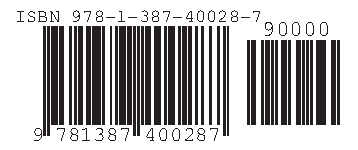
\includegraphics{isbn_barcode}

\closeout\chapterlist
\end{document}
